\section{Verification, stress tests, and interpretation of the figures}
\label{sec:verification}

Verification has three distinct layers. First, the pinned workbench contains written model-specific derivations and source-bound historical admission records. Second, the Round26 release was replayed from a clean detached tree: 40 current producer executions and four inherited AA executions covered normal and optimized Python, 171 admission mutations were rejected in each mode, 156 generated files were compared, and seven interface suites passed. These are evidence of reproducibility and admission integrity, not a proof-assistant verification of the mathematics. Third, this manuscript adds a separately authored mathematical stress suite and parameterized calculators. Repeated execution in another interpreter mode is not counted as an additional independent derivation.

\subsection{What the new checks challenge}
The fresh calculator suite passes 194 checks; the separately authored skeptic suites pass 158 checks (90 general, 12 early, 33 middle, and 23 recent). Each corresponding normal and optimized Python run has identical result bytes. The standalone HTML formulas pass 15 additional checks. These are distinct programmed checks, not counts of independently proved theorems or measures of statistical confidence.

The independent skeptic suite derives selected identities without importing the producer implementations. It checks normalized Haar moments and their differential recurrence, tests a false moment closure, distinguishes two-trace from three-trace information, reconstructs the shared-link mixed derivative, enumerates the two-square shell minima, and recertifies the one-square continuous gap through a separate rational Sturm and full-tail argument. Further tests expose delayed omitted-channel loading, distinguish a source identity from an operator identity, count translated boundary crossings, check Wilson spectral moments and phase signs, and verify the rational preparation and combined AF2 error budgets. The audit ledger records which manuscript contributions were reviewed and which historical production runs were not rerun.

The calculator tests compare independent numerical representations where available: Bessel ratios against normalized Haar quadrature, matrix dimensions against one another as diagnostics, exact rational enclosures against the recorded coefficients, and boundary or invalid inputs against the declared domains. These tests deliberately include wrong models. For example, an approximation that drops variance can pass a selected equation and still fail the next moment identity. A retained initial column equal to zero can coexist with nonzero later leakage. A ground-energy rounding error can pass short-time tests and fail at sufficiently long times.

\subsection{Arithmetic, analytic scope, and sampling}
Exact rational arithmetic certifies the arithmetic statement it evaluates. It does not make an unevaluated transcendental quantity exact; such a quantity needs a proved enclosure. The companion distinguishes positive Taylor partial sums used as rigorous exponential bounds from high-precision floating diagnostics. Jacobi truncation comparisons are labelled diagnostics unless a separate omitted-tail and interval argument is invoked. The HTML calculators use ordinary double precision and display rounded values; they are explanatory interfaces to the formulas, not interval-proof engines.

A plot samples a formula. Its visual smoothness supplies no all-time, all-coupling, or infinite-volume proof. Uniform bounds in the paper come from the stated analytic arguments: complete interval coverage with a continuity estimate, a monotone early/late envelope, a convergent majorant, or a complete spectral/channel identity. Each plot states its parameter region and whether it shows an exact function, a sufficient upper budget, or numerical diagnostic data.

\subsection{Known limits of this audit}
Neither this manuscript audit nor a finite set of stress tests can establish that the work has no limitations or that every possible error has been excluded. The complete historical numerical production archive was not regenerated for this paper. The source checkpoint, original reports, fresh calculation scripts, source hashes, and per-contribution dispositions make that boundary inspectable. No unrestricted continuum conclusion is admitted by inference from the calculations. No experimental application, literature priority, or external peer-review status is claimed.

\begin{figure}[htbp]\centering
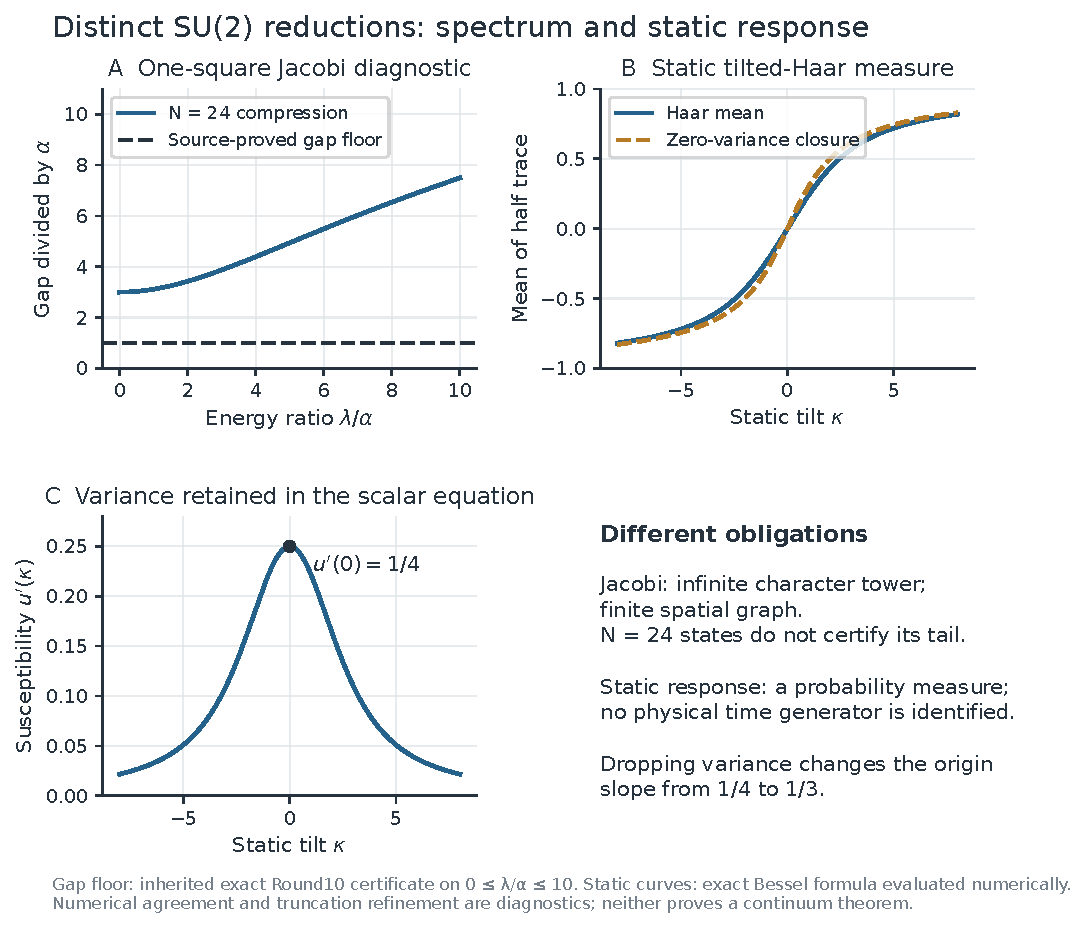
\includegraphics[width=\textwidth]{figures/jacobi_static.pdf}
\caption{Two distinct benchmarks. The one-square Jacobi eigenvalue curves are finite-matrix numerical diagnostics; the recorded continuous full-space certificate has its own tail and interval proof. The tilted-Haar mean and variance are static quantities, not a physical trajectory. Plot data and parameters are supplied with the calculators.}
\label{fig:jacobi-static}
\end{figure}

\begin{figure}[htbp]\centering
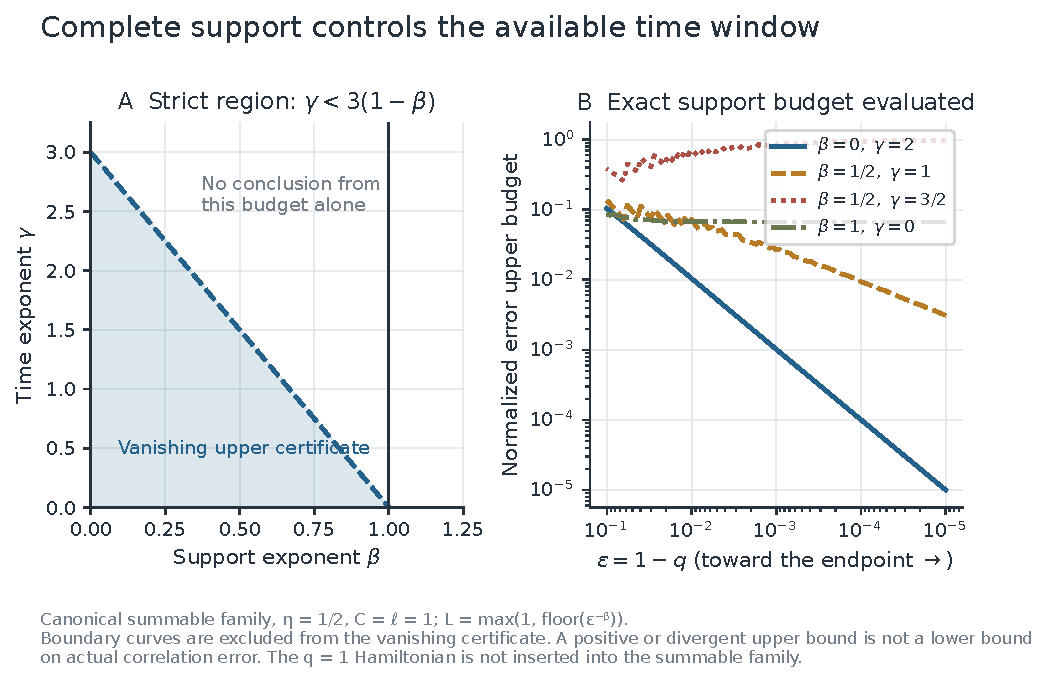
\includegraphics[width=\textwidth]{figures/support_window.pdf}
\caption{Sufficient support/time windows and evaluated upper budgets. The strict exponent region follows from the stated complete-support asymptotics. Values outside it indicate failure of this sufficient certificate, not proof that the actual correlation error diverges.}
\label{fig:support-window}
\end{figure}

\begin{figure}[htbp]\centering
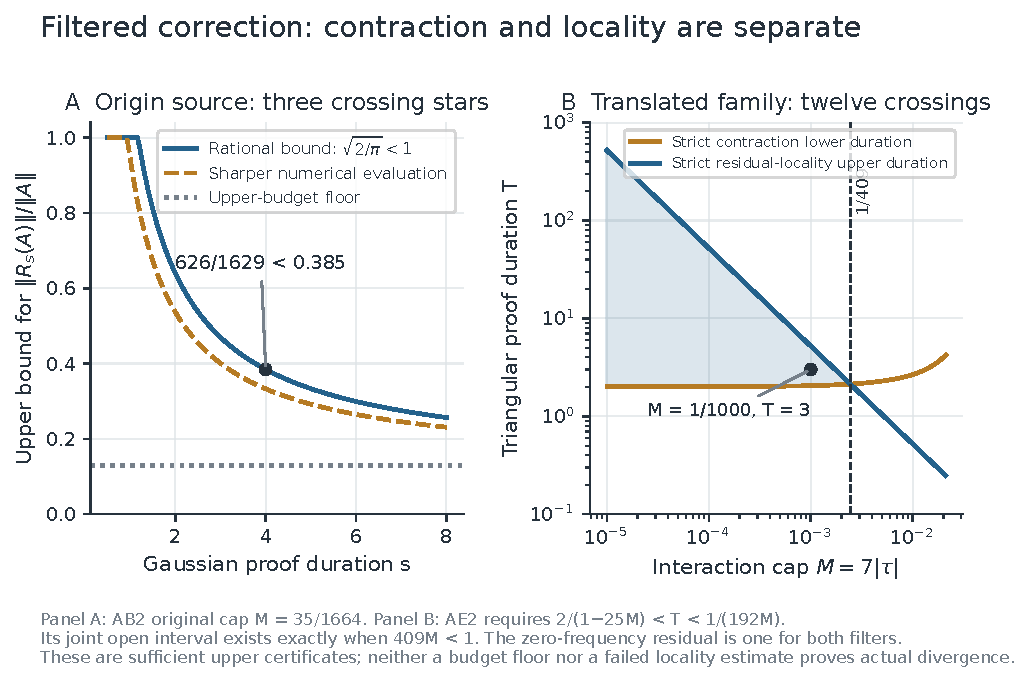
\includegraphics[width=\textwidth]{figures/filter_budgets.pdf}
\caption{Full-source Gaussian contraction and compact-filter certificate compatibility. Gaussian duration is a proof regulator. The compact construction has a smaller admitted coupling range and counts all translated crossings. The original-cap incompatibility concerns these sufficient bounds, not every possible filter or a lower bound on an actual error.}
\label{fig:filter-budgets}
\end{figure}

\begin{figure}[htbp]\centering
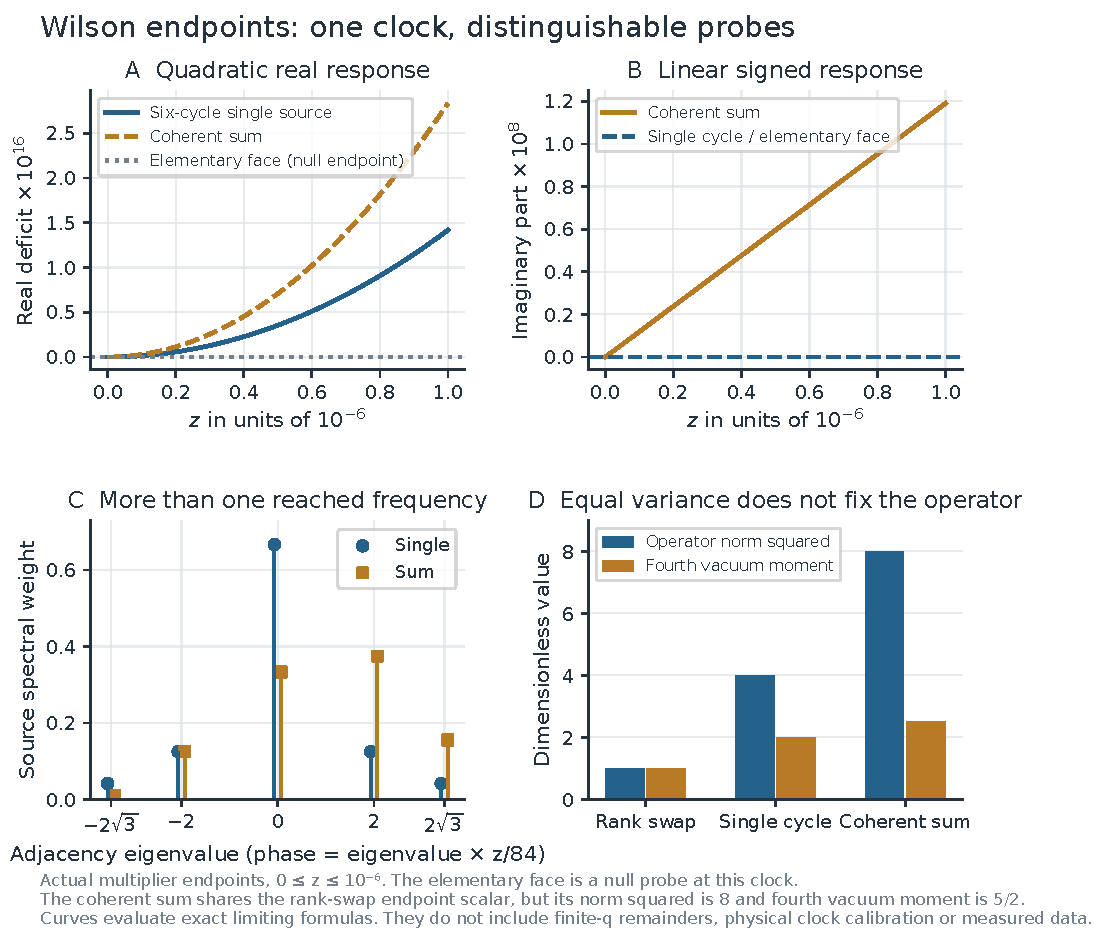
\includegraphics[width=\textwidth]{figures/wilson_endpoints.pdf}
\caption{Canonical endpoint functions for the specified actual Wilson observables, their reached spectral weights, and distinctions between operator norms and moments. The elementary probe supplies a null slow-response control. These are model readouts; finite-$q$ deviations and physical resource costs require their separate bounds.}
\label{fig:wilson-endpoints}
\end{figure}

\begin{figure}[htbp]\centering
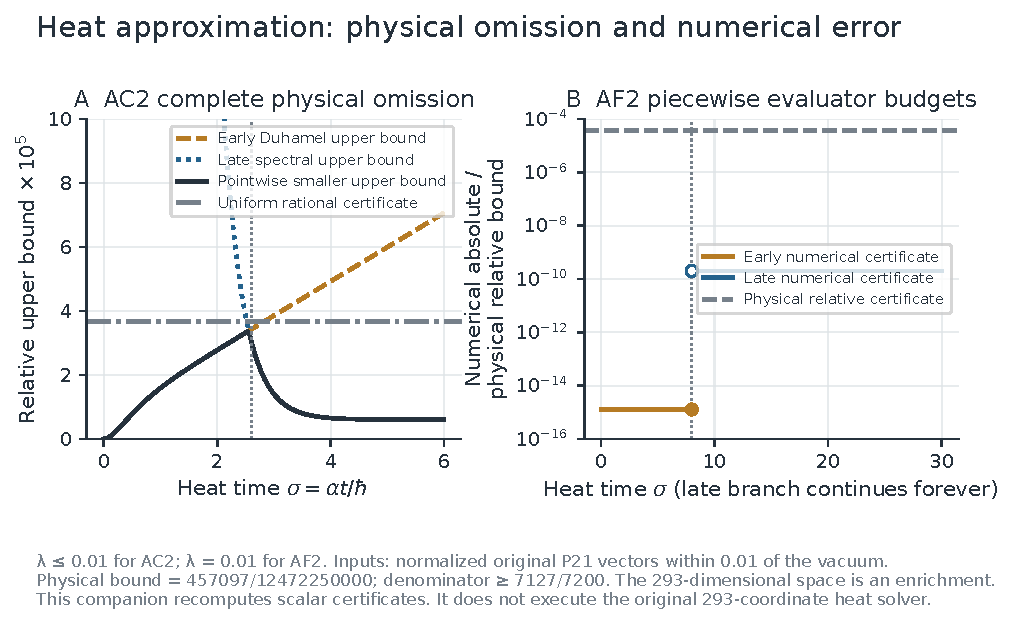
\includegraphics[width=\textwidth]{figures/heat_certificates.pdf}
\caption{The physical AC2 early/late envelope and the separately charged AF2 numerical bound. The numerical branch changes at $\sigma=8$ to prevent secular center error. The denominator applies to the original normalized $P_{21}$ preparation ball; no relative claim for arbitrary ground-null inputs is shown. The late branch extends to all later times even though the horizontal display ends.}
\label{fig:heat-certificates}
\end{figure}

